% Micro Speed Grader: user manual (DRAFT).
% The chapters are generated from the in-app help (docs/help/*.md) by app/scripts/manual.ts:
%   cd app && npm run manual
% Edit the help pages, not chapters/*.tex. This file holds the layout, the cover and the key caps.
\documentclass[10pt]{article}
\usepackage[margin=0.75in]{geometry}
\usepackage[T1]{fontenc}
\usepackage{lmodern}
\usepackage{microtype}
\usepackage{booktabs}
\usepackage[table]{xcolor}
\usepackage{enumitem}
\usepackage{fancyhdr}
\input{version}
\newcommand{\manualauthors}{Gadin and Le}
\pagestyle{fancy}
\fancyhf{}
\fancyhead[L]{Micro Speed Grader}
\fancyhead[C]{User Manual \textcolor{draftred}{(Draft)}}
\fancyhead[R]{Version \appversion}
\fancyfoot[L]{}
\fancyfoot[C]{\thepage}
\fancyfoot[R]{}
\setlength{\headheight}{15pt}
\renewcommand{\headrulewidth}{0.4pt}
\renewcommand{\footrulewidth}{0.4pt}
\definecolor{accent}{HTML}{1F4E79}
\definecolor{soft}{HTML}{E8EEF5}
\definecolor{draftred}{HTML}{B03A2E}
\setlist{nosep,leftmargin=1.2em}
\setlength{\parindent}{0pt}
\setlength{\parskip}{4pt}
\usepackage{tikz}
\usepackage{amssymb}
\usepackage{graphicx}
\usepackage[most]{tcolorbox}
\usepackage{tabularx}
\newcolumntype{Y}{>{\raggedright\arraybackslash}X}
\usetikzlibrary{calc}

% ---- added for the manual ----
\usepackage{textcomp}
\usepackage{pifont}
\usepackage{alltt}
\usepackage{qrcode}
\usepackage{titlesec}
\usepackage{draftwatermark}
\SetWatermarkText{DRAFT}
\SetWatermarkScale{1.1}
\SetWatermarkColor[gray]{0.94}
\usepackage[hidelinks]{hyperref}
\hypersetup{colorlinks=true, linkcolor=accent, urlcolor=accent, pdftitle={Micro Speed Grader: User Manual (Draft, version \appversion)}}
\setcounter{tocdepth}{1}
\makeatletter\renewcommand*\l@subsection{\@dottedtocline{2}{1.5em}{2.6em}}\makeatother
\titleformat{\section}{\Large\bfseries\color{accent}}{\thesection}{0.6em}{}
\titleformat{\subsection}{\large\bfseries}{\thesubsection}{0.6em}{}
\titleformat{\subsubsection}{\normalsize\bfseries}{\thesubsubsection}{0.6em}{}
\titlespacing*{\section}{0pt}{18pt}{6pt}
\titlespacing*{\subsection}{0pt}{12pt}{3pt}

% key caps: one rounded box per key
\newtcbox{\keycap}{enhanced, on line, nobeforeafter, tcbox raise base, boxsep=0pt, left=2.6pt, right=2.6pt, top=1.4pt, bottom=1.4pt,
  arc=2.4pt, boxrule=0.45pt, bottomrule=1.1pt, colback=white, colframe=black!38, fontupper=\footnotesize\sffamily}
\newcommand{\keyplus}{\kern1.5pt}
% symbols drawn so any LaTeX engine can typeset them
\newcommand{\cmdsym}{\tikz[baseline=-0.6ex, x=0.3em, y=0.3em, line width=0.38pt]{%
  \draw (-0.32,-0.32) rectangle (0.32,0.32);
  \foreach \sx/\sy in {1/1,-1/1,-1/-1,1/-1} \draw (0.32*\sx+0.24*\sx,0.32*\sy+0.24*\sy) circle (0.26);}}
\newcommand{\optsym}{\tikz[baseline=-0.1ex, x=0.55em, y=0.55em, line width=0.45pt]{\draw (0,0.8) -- (0.35,0.8) -- (0.8,0) -- (1.15,0); \draw (0.7,0.8) -- (1.15,0.8);}}
\newcommand{\shiftsym}{\tikz[baseline=-0.1ex, x=0.5em, y=0.5em, line width=0.45pt]{\draw (0.3,0) -- (0.3,0.45) -- (0,0.45) -- (0.6,1.1) -- (1.2,0.45) -- (0.9,0.45) -- (0.9,0) -- cycle;}}
\newcommand{\returnsym}{\ensuremath{\hookleftarrow}}
\newcommand{\deletesym}{\textsf{Delete}}
\newcommand{\tabsym}{\textsf{Tab}}
\newcommand{\menuarrow}{\,\raisebox{0.15ex}{\scalebox{0.7}{\ensuremath{\blacktriangleright}}}\,}
\newcommand{\checksym}{\ding{51}}
\newcommand{\crosssym}{\ding{55}}
\newcommand{\warnsym}{\tikz[baseline=-0.1ex, x=0.6em, y=0.6em]{\draw[line width=0.45pt, line join=round] (0,0) -- (1,0) -- (0.5,0.9) -- cycle; \node[font=\tiny\bfseries, inner sep=0] at (0.5,0.32) {!};}}

% boxes
\newtcolorbox{note}{enhanced, breakable, colback=soft, colframe=soft, boxrule=0pt, borderline west={2.2pt}{0pt}{accent},
  arc=2pt, left=8pt, right=8pt, top=5pt, bottom=5pt, before skip=8pt, after skip=8pt}
\newtcolorbox{codebox}{enhanced, breakable, colback=black!3, colframe=black!12, boxrule=0.4pt, arc=3pt, left=8pt, right=8pt, top=4pt, bottom=4pt,
  fontupper=\small, before skip=8pt, after skip=8pt}
\newtcolorbox{pagecard}{enhanced, sidebyside, sidebyside align=center, lefthand ratio=0.8, segmentation hidden, colback=white,
  colframe=black!14, boxrule=0.5pt, arc=4pt, left=9pt, right=9pt, top=7pt, bottom=7pt, before skip=6pt, after skip=6pt, breakable=false}
\newcommand{\onlinemark}{\raisebox{0.1ex}{\scalebox{0.7}{\ensuremath{\nearrow}}}}
% figures: the screenshot with rounded corners, the caption under it
\newcommand{\shot}[3]{% width, file, caption
  \par\begin{center}
  \tcbox[enhanced, boxsep=0pt, left=0pt, right=0pt, top=0pt, bottom=0pt, arc=5pt, boxrule=0.5pt, colframe=black!22, colback=white, clip upper]%
    {\includegraphics[width=#1, height=0.27\textheight, keepaspectratio]{#2}}\par\vspace{2pt}
  {\footnotesize\color{black!60}#3}
  \end{center}\par}

\begin{document}

% ---------------- cover ----------------
\begin{titlepage}
\thispagestyle{empty}
\SetWatermarkText{}
\begin{tikzpicture}[remember picture, overlay]
  \fill[accent] (current page.north west) rectangle ($(current page.north east)+(0,-7.2cm)$);
  \fill[soft] ($(current page.north west)+(0,-7.2cm)$) rectangle ($(current page.north east)+(0,-7.45cm)$);
  \node[anchor=north west, inner sep=0] at ($(current page.north west)+(2cm,-1.7cm)$) {\includegraphics[width=2.6cm]{icon.png}};
  \node[anchor=north west, align=left, text=white, inner sep=0] at ($(current page.north west)+(5.2cm,-1.9cm)$)
    {{\fontsize{30}{34}\selectfont\bfseries Micro Speed Grader}\\[10pt]{\Large User Manual}};
  \node[anchor=north west, inner sep=0] at ($(current page.north west)+(5.2cm,-4.6cm)$)
    {\tcbox[colback=draftred, colframe=draftred, arc=3pt, boxsep=2pt, left=6pt, right=6pt, fontupper=\color{white}\bfseries\large]{DRAFT}};
  \node[anchor=north west, inner sep=0, text=white] at ($(current page.north west)+(7.8cm,-4.72cm)$)
    {\large For version \appversion};
\end{tikzpicture}
\vspace*{6.6cm}

{\large Grade virtual-microscopy practicals one question at a time.}

\vspace{6pt}
Students drop a pin on a structure in a whole-slide image. Micro Speed Grader gathers every student's pin for a question onto one slide, groups pins that land on the same structure, and lets you grade a whole group with one key press. When you're done it exports a grades spreadsheet and a feedback note for each student.

\vspace{14pt}
\begin{tcolorbox}[colback=white, colframe=draftred!70, boxrule=0.6pt, arc=3pt, left=10pt, right=10pt, top=8pt, bottom=8pt]
\textbf{\color{draftred}This is a draft.} It describes \textbf{Micro Speed Grader \appversion}\appchanges. Built \builddate{} from commit \texttt{\appcommit}. Details and screenshots may change before the final version. The Help built into the app (\textbf{Help} in the menu bar, or the \keycap{?}\ button) is always up to date.
\end{tcolorbox}

\vfill
\begin{center}
\begin{tabular}{@{}c@{\hspace{2.6cm}}c@{}}
\href{\repourl}{\qrcode[height=3cm, nolink]{\repourl}} & \href{\releaseurl}{\qrcode[height=3cm, nolink]{\releaseurl}}\\[6pt]
\textbf{Source code and help} & \textbf{Download the app}\\
\href{\repourl}{\small\texttt{github.com/agadin/micro-speed-grader}} & \href{\releaseurl}{\small\texttt{\ldots/releases/latest}}\\[2pt]
{\footnotesize\color{black!60}issues, the online help, the code} & {\footnotesize\color{black!60}macOS (Apple silicon and Intel) and Windows}
\end{tabular}
\end{center}
\vspace{1.2cm}
{\small\color{black!60}\manualauthors\hfill \builddate}
\end{titlepage}

% ---------------- contents ----------------
\SetWatermarkText{DRAFT}
\tableofcontents
\vspace{10pt}
\begin{note}
\textbf{About this manual.} The first sections cover everyday grading in full: setting up, grading, selecting pins, the answer key and exporting. \hyperref[sec:more]{More in the online help} summarises the rest (working with other graders, editing exam questions, the ledger, preferences, troubleshooting and more), each with a QR code to its full page. Links marked \onlinemark{} open the online help. On Windows, use \keycap{Ctrl} where this manual shows \keycap{\cmdsym}, and \keycap{Alt} for \keycap{\optsym}.
\end{note}
\clearpage

\section{Introduction}\label{sec:index}

\phantomsection\label{sec:index:micro-speed-grader-help}

Micro Speed Grader marks virtual-microscopy practicals one question at a time. Students drop a pin on a structure in a whole-slide image. The app gathers every student's pin for a question onto one slide, groups pins that land on the same structure, and lets you grade a whole group with one key press. When you're done it exports a grades spreadsheet and a feedback note for each student.

\begin{figure}[H]\centering\framedshot{0.72\linewidth}{img/grading-overview.jpg}\caption{The grading screen: one question, every student's pins, grouped into clusters}\label{fig:overview}\end{figure}
\vspace{-10pt}
\begin{note}Hover over any control in the app to see what it does. When the tooltip shows a \keycap{?}, click it to jump to the matching section here.\end{note}
\vspace{-10pt}
\section{Getting started}\label{sec:getting-started}

\phantomsection\label{sec:getting-started:getting-started}

\subsection{What you need}\label{sec:getting-started:what-you-need}

\begin{itemize}[topsep=2pt, itemsep=2pt]
\item \textbf{The exam}: the exam PDF, or a JSON file listing the questions. Each question names the slide (or slides) it uses, for example \texttt{Q1. Using VMS109, place a pin on an eccrine sweat gland}.
\item \textbf{The student submissions folder}: one folder per student, each holding that student's \texttt{.ndpa} annotation files (the pins they placed in NDP.view).
\item \textbf{The slides folder}: the whole-slide images the exam uses (\texttt{.ndpi}, \texttt{.svs}, \texttt{.tif}, \texttt{.tiff}, \texttt{.mrxs}, \texttt{.scn} or \texttt{.vms}). File names must contain the slide ID, such as \texttt{VMS109}.
\end{itemize}

\subsection{The start screen}\label{sec:getting-started:the-start-screen}

\begin{figure}[H]\centering
\subshot[fig:start-screen]{0.3}{img/start.png}{The start screen}\hspace{0.06\linewidth}%
\subshot[fig:new-session]{0.55}{img/new-session.png}{Setting up a new session}
\caption{Starting out}\label{fig:start}
\end{figure}

The start screen (Figure~\ref{fig:start-screen}) offers:

\begin{itemize}[topsep=2pt, itemsep=2pt]
\item \textbf{New grading session\ldots{}} sets up a new session from the three things above.
\item \textbf{Open session\ldots{}} opens a \texttt{.msgrade} session file.
\item \textbf{Resume} lists the last ten sessions you opened, with when each was last saved. Click one to carry on; the \textbf{\ensuremath{\times}} only removes it from the list (the file stays where it is).
\item \textbf{Got work from another grader?} opens a hand-off pack someone sent you. See \hyperref[sec:handoff]{Grade with other people}.
\end{itemize}

\subsection{Create a session}\label{sec:getting-started:create-a-session}

The \textbf{New grading session} window (Figure~\ref{fig:new-session}) takes you through five steps:

\begin{enumerate}[topsep=2pt, itemsep=2pt]
\item \textbf{Exam questions}: click \textbf{Choose exam PDF / JSON\ldots{}}. To fix what was read, or to add questions it missed, click \textbf{Edit questions\ldots{}} (see \href{https://github.com/agadin/micro-speed-grader/blob/main/docs/help/exam-questions.md}{Set up exam questions}\,\onlinemark{}). No exam file? Choose \textbf{Set up the questions by hand}. The app reads every line shaped like \texttt{Q1. Using VMS123, \ldots{}} and lists the questions in a table. Edit the session name if you like.
\item \textbf{Student submissions folder}: click \textbf{Choose folder\ldots{}} and pick the folder that holds one folder per student. The app shows how many student folders and annotation files it found.
\item \textbf{Slide images folder}: click \textbf{Choose folder\ldots{}} and pick the folder of slides. Each question's slides are marked \textbf{\checksym{}} when found or \textbf{missing} when not.
\item \textbf{Save session as}: click \textbf{Choose\ldots{}} and pick where to keep the session file. It's pre-filled next to the submissions folder.
\item Click \textbf{Start grading \ensuremath{\rightarrow}}.
\end{enumerate}

\textbf{Start grading \ensuremath{\rightarrow}} stays greyed out until at least one question is included and all three folders and the save location are chosen. Until then, the line next to it says what's still needed (hover over the button for the same list).

\subsubsection{Choosing which questions to grade}\label{sec:getting-started:choosing-which-questions-to-grade}

The table has a checkbox per question. Choosing the slides folder ticks only the questions whose slides were found. Untick a question to leave it out; the score is out of the number of included questions (shown under the table as \emph{N of M questions included}).

You can correct the \textbf{Slides} cell if the exam lists the wrong slide ID: type the IDs separated by commas or spaces.

How the app works out which student, slide and question each pin belongs to is described in Appendix~\ref{app:pins}.

\subsubsection{Answer key (optional)}\label{sec:getting-started:answer-key-optional}

The last step lets you import an \hyperref[sec:answer-key]{answer key} saved from another session, or start by marking one. Pins that land in the key's areas are graded for you.

\subsection[Things to check\alsotoc{sec:getting-started:saving-and-backups}{Saving and backups}]{Things to check}\label{sec:getting-started:things-to-check}

Once the exam and the submissions folder are chosen, the app reads every student's files. If anything looks wrong, step 2 shows \textbf{\warnsym{} N things to check \textperiodcentered{} Review}. Click \textbf{Review} to see each problem, what it means and what to do, with the students and files it affects. Long lists are cut short: click \textbf{Show all} to see the rest.

The top of the list shows how far you've got: how many were found, fixed, acknowledged and left. Work through it like this:

\begin{itemize}[topsep=2pt, itemsep=2pt]
\item \textbf{This file is for\ldots{}}: for a file with no slide ID, or the wrong one, choose the slide it's really for. The app reads it as that slide from then on (including when you \href{https://github.com/agadin/micro-speed-grader/blob/main/docs/help/getting-started.md\#new-and-changed-submissions}{rescan}\,\onlinemark{}); the file itself isn't renamed. It moves to \textbf{Fixed}, where \textbf{Undo} takes it back.
\item \textbf{Show file} / \textbf{Show folder} opens it in Finder, so you can look at it or add what's missing. Then click \textbf{Check again}.
\item \textbf{OK} marks one item as checked; \textbf{Acknowledge all} does a whole group, or everything left. Acknowledged items stay listed, crossed out, and \textbf{Undo} puts one back.
\end{itemize}

When nothing is left, step 2 shows \textbf{\checksym{} All N checked}. You can start grading at any time, whether or not everything is checked. Fixes and acknowledgements are saved with the session.

\begingroup\renewcommand{\arraystretch}{1.35}
\noindent\begin{tabularx}{\linewidth}{YYY}
\toprule
\textbf{Problem} & \textbf{What it means} & \textbf{What to do} \\
\midrule
\textbf{Nothing to grade} & A student's folder has no pins the app can use (no \texttt{.ndpa} files, or none for the exam's slides). & Check whether the student submitted. If they did, put their \texttt{.ndpa} files in their folder. \\
\textbf{Missing a slide} & The student has no file for a slide an included question uses, so they have no answer for it. & If the file is there under another name, rename it so it includes the slide ID. \\
\textbf{No slide ID in the file name} & The app can't tell which slide the file is for, so its pins are left out. & Rename the file so it includes the slide ID, e.g. \texttt{VMS109.ndpi.ndpa}. \\
\textbf{Slide not in the exam} & No question uses that slide, so its pins are left out. & Usually nothing. If the student typed the wrong slide ID, rename the file. \\
\textbf{Pin names a question not on that slide} & A pin titled, say, \emph{Q9} is on a slide that's only for Q2. It's still graded with that slide's questions. & Look at it when you grade that slide: the student may have mislabelled the pin or used the wrong slide. \\
\textbf{Too many pins} & Only the first 50 pins per student per slide are kept. & Open the file in NDP.view if you need the rest. \\
\textbf{File too large} & Annotation files over 2 MB are skipped; a real one is a few KB. & It's probably damaged. Ask the student to save it again from NDP.view. \\
\textbf{File can't be read} & The file isn't valid annotation data, so it was skipped. & Ask the student to save it again from NDP.view. \\
\bottomrule
\end{tabularx}\endgroup\par\medskip

Files for a question you've left out (unticked) aren't checked.

\tocoff
\subsection{Saving and backups}\label{sec:getting-started:saving-and-backups}
\tocon

There's no Save button: the session saves itself a moment after every change, and whenever you change image or close the session. The top bar shows \textbf{Saving\ldots{}}, then \textbf{\checksym{} Saved}.

Each save keeps the previous version next to it as \texttt{yoursession.msgrade.bak}. If the session file is ever damaged, opening it falls back to the backup automatically.

To stop for the day, click the close button at the right of the top bar (\textbf{Save and close session}). Next time, click the session under \textbf{Resume}.

{\small\textbf{Also in the online help:} \href{https://github.com/agadin/micro-speed-grader/blob/main/docs/help/getting-started.md\#new-and-changed-submissions}{New and changed submissions}\,\onlinemark{} \textperiodcentered{} \href{https://github.com/agadin/micro-speed-grader/blob/main/docs/help/getting-started.md\#review-changed-submissions}{Review changed submissions}\,\onlinemark{} \textperiodcentered{} \href{https://github.com/agadin/micro-speed-grader/blob/main/docs/help/getting-started.md\#updates}{Updates}\,\onlinemark{}}

\section{Grading}\label{sec:grading}

\phantomsection\label{sec:grading:grading}

You grade one \textbf{image} at a time: one question on one slide, with every student's pin for that question. Pins that sit close together are grouped into \textbf{clusters}, biggest first, so the common answers come up first and you can grade dozens of students with one key.

\shot{0.36\linewidth}{img/grade-cluster.png}{Grading a cluster: select, then C for correct or W for wrong with a reason}

\subsection{The grading screen}\label{sec:grading:the-grading-screen}

The grading screen (Figure~\ref{fig:overview}) has five parts:

\begin{itemize}[topsep=2pt, itemsep=2pt]
\item \textbf{Top bar}: the session name, the image menu (\emph{Q1 \textperiodcentered{} VMS109}, with \emph{image 2 of 5} below it), undo and redo, the save status, \textbf{Find student} (see \href{https://github.com/agadin/micro-speed-grader/blob/main/docs/help/students.md}{Look up a student}\,\onlinemark{}), \textbf{Hand off}, \textbf{Export}, Preferences, help and close.
\item \textbf{The slide}, with the students' pins, the current cluster's dashed ring, a minimap (top left) and a scale bar.
\item \textbf{Bottom toolbar}: previous/next cluster, how many pins are selected, \textbf{Correct}, \textbf{Wrong\ldots{}}, the \textbf{Whole slide / Cluster} zoom switch and \textbf{Shortcuts}.
\item \textbf{Right panel}: the question text, cluster settings, selection tools, display options, recent reasons and progress. Click a section's heading to fold it away.
\item \textbf{Ledger} (bottom): every grade you've given. See \href{https://github.com/agadin/micro-speed-grader/blob/main/docs/help/ledger.md}{The ledger and undo}\,\onlinemark{}.
\end{itemize}

\subsection{Grade a cluster}\label{sec:grading:grade-a-cluster}

The app opens on the biggest cluster and selects its ungraded pins.

\begin{enumerate}[topsep=2pt, itemsep=2pt]
\item Look at what the pins in the ring are on. Zoom with the scroll wheel; \keycap{F} zooms back to the cluster, \keycap{H} shows the whole slide.
\item If they're right, press \keycap{C} (or click \textbf{Correct}). They turn green and the next cluster comes up.
\item If they're wrong, press \keycap{W} (or click \textbf{Wrong\ldots{}}), type what they marked instead (for example \emph{Neutrophil}) and press \keycap{\returnsym{}}. That reason goes into those students' feedback.
\item When the ring holds a mix, select just the right pins first, with the lasso, brush or polygon. See \hyperref[sec:selecting]{Selecting pins}.
\end{enumerate}

Press \keycap{]} to skip to the next cluster and \keycap{[} to go back. When an image is done, the next image comes up from the \textbf{Next image} button or \keycap{\cmdsym{}}\keyplus{}\keycap{\ensuremath{\rightarrow}}.

\subsubsection{Correct with a note}\label{sec:grading:correct-with-a-note}

\keycap{\shiftsym{}}\keyplus{}\keycap{C} (or \shiftsym{}-click \textbf{Correct}) marks the selection correct and lets you add a note, such as \emph{Correct, but borderline}. The note shows in the student's feedback as \emph{Correct (note)}.

\subsection[The grade menu\alsotoc{sec:grading:reasons-for-wrong-answers}{Reasons for wrong answers}]{The grade menu}\label{sec:grading:the-grade-menu}

\begin{figure}[H]\centering
\subshot[fig:grade-menu]{0.3}{img/grade-menu.jpg}{The grade menu}\hspace{0.06\linewidth}%
\subshot[fig:reason-box]{0.3}{img/reason-box.jpg}{Giving a reason}
\caption{Grading the selection}\label{fig:grade}
\end{figure}

Click a pin, press \keycap{\returnsym{}}, or right-click without dragging to open the grade menu for the selection (Figure~\ref{fig:grade-menu}):

\begingroup\renewcommand{\arraystretch}{1.35}
\noindent\begin{tabularx}{\linewidth}{YYY}
\toprule
\textbf{Item} & \textbf{Key} & \textbf{What it does} \\
\midrule
Mark correct & C & Grade the selection correct \\
Correct with note\ldots{} & \shiftsym{}C & Correct, with a note for the student \\
Mark wrong\ldots{} & W & Grade it wrong and give a reason \\
Invert selection & X & Select the other ungraded pins on this image instead \\
Isolate & I & Hide every other pin \\
Remove grade & U & Make the selected pins ungraded again \\
Close & Esc & Close the menu \\
\bottomrule
\end{tabularx}\endgroup\par\medskip

\tocoff
\subsection{Reasons for wrong answers}\label{sec:grading:reasons-for-wrong-answers}
\tocon

When you mark pins wrong, the reason box (Figure~\ref{fig:reason-box}) suggests reasons you've used before: this question's first, then the rest of the exam.

\begin{itemize}[topsep=2pt, itemsep=2pt]
\item Press \keycap{1}--\keycap{9} (on an empty box) to pick a suggestion, or \keycap{\cmdsym{}}\keyplus{}\keycap{1}--\keycap{\cmdsym{}}\keyplus{}\keycap{9} while typing.
\item \keycap{\ensuremath{\uparrow}} \keycap{\ensuremath{\downarrow}} highlight a suggestion and \keycap{\tabsym{}} completes it.
\item \keycap{\returnsym{}} applies, \keycap{Esc} goes back.
\end{itemize}

The \textbf{Recent reasons} section of the right panel lists this question's last few reasons with how many pins each has. Click one to mark the current selection wrong with that reason.

By default a reason is required. To allow blank reasons (students then read \emph{Incorrect}), turn off \textbf{Wrong answers need a reason} in \href{https://github.com/agadin/micro-speed-grader/blob/main/docs/help/preferences.md\#grading-text}{Preferences \menuarrow{} Grading text}\,\onlinemark{}.

\subsection{Pins that grade themselves}\label{sec:grading:pins-that-grade-themselves}

\begin{itemize}[topsep=2pt, itemsep=4pt]
\item \phantomsection\label{sec:grading:double-pins}\textbf{Double pins.} A student who placed more than one pin for the same question gets a \keycap{2} badge on their pins. They're counted as done and marked wrong with \emph{Multiple pins submitted (only one allowed)}, shown in the ledger as an \textbf{AUTO} row. If you grade one of their pins yourself, your most recent grade counts instead.
\item \phantomsection\label{sec:grading:no-answer}\textbf{No answer.} A student with no pin for a question is marked wrong with \emph{No answer} in the export. There's nothing to grade on the slide.
\item \phantomsection\label{sec:grading:unlabelled-pins}\textbf{Unlabelled pins (\keycap{?}).} A pin whose title doesn't say which question it answers, on a slide that several questions use, shows a \keycap{?} badge and appears on each of those questions. Grade it on the question it answers: that also assigns it. \textbf{Remove grade} undoes the assignment. See Appendix~\ref{app:pins}.
\end{itemize}

\subsection{Progress}\label{sec:grading:progress}

The \textbf{Progress} section shows three bars: \textbf{This image}, \textbf{Images done} and \textbf{All pins}. When every pin is graded a banner offers \textbf{Export grades}. See \hyperref[sec:export]{Exporting grades}.

{\small\textbf{Also in the online help:} \href{https://github.com/agadin/micro-speed-grader/blob/main/docs/help/grading.md\#showing-the-pins-differently}{Showing the pins differently}\,\onlinemark{}}

\section{Selecting pins}\label{sec:selecting}

\phantomsection\label{sec:selecting:selecting-pins}

Usually the app's cluster selection is all you need: press \keycap{C} or \keycap{W}. When a cluster holds a mix of right and wrong answers, select the pins yourself first. Turn tools on and off in \href{https://github.com/agadin/micro-speed-grader/blob/main/docs/help/preferences.md\#selection}{Preferences \menuarrow{} Selection}\,\onlinemark{}.

\subsection[The mouse\alsotoc{sec:selecting:lasso}{Lasso, brush and polygon}]{The mouse}\label{sec:selecting:the-mouse}

By default the \textbf{right} button selects and the \textbf{left} button pans the slide. Swap them in \href{https://github.com/agadin/micro-speed-grader/blob/main/docs/help/preferences.md\#mouse--keys}{Preferences \menuarrow{} Mouse \& keys}\,\onlinemark{} (\textbf{Left selects}). Scroll to zoom.

When more than one tool is on, the \textbf{Select} section of the right panel shows a switcher. \keycap{B} cycles through the tools.

\tocoff
\subsection{Lasso, brush and polygon}\label{sec:selecting:lasso}
\tocon\label{sec:selecting:brush}\label{sec:selecting:polygon}

\begin{figure}[H]\centering
\subshot{0.32}{img/lasso-use.png}{Lasso}\hfill
\subshot{0.32}{img/brush-use.png}{Brush}\hfill
\subshot{0.32}{img/polygon-use.png}{Polygon}
\caption{The three selection tools, partway through selecting some of a cluster's pins}\label{fig:tools}
\end{figure}

{\setlist[itemize]{leftmargin=1em, topsep=3pt, itemsep=2pt, after=\vspace{-\baselineskip}}
\noindent\begin{tabularx}{\linewidth}{@{}Y@{\hspace{1.2em}}Y@{\hspace{1.2em}}Y@{}}
\toprule
\textbf{Lasso} & \textbf{Brush} & \textbf{Polygon} \\
\midrule
Drag a loop around the pins. When you let go, the grade menu opens beside them.
\begin{itemize}
\item \keycap{\cmdsym{}}-drag adds to the selection (the menu stays closed).
\item \keycap{\shiftsym{}}-drag selects everything \emph{outside} the loop.
\item \keycap{\optsym{}}-drag draws a rectangle.
\item \keycap{\cmdsym{}}-click a pin adds or removes just that pin.
\item \keycap{X} inverts the selection.
\end{itemize}
&
Paint over the pins. Painting replaces the selection and opens the menu.
\begin{itemize}
\item \keycap{\shiftsym{}} adds and \keycap{\optsym{}} removes, without opening the menu.
\item \keycap{-} and \keycap{=} make the brush smaller or bigger. The size slider is in the \textbf{Select} section.
\end{itemize}
&
Click to place corners around the pins. Close the shape by clicking the first corner, double-clicking, or pressing \keycap{\returnsym{}}.
\begin{itemize}
\item \keycap{\deletesym{}} removes the last corner; \keycap{Esc} cancels.
\item \keycap{\cmdsym{}} on the first click adds to the selection; \keycap{\shiftsym{}} selects the outside.
\end{itemize}
\\
\bottomrule
\end{tabularx}}\par\medskip

{\small\textbf{Also in the online help:} \href{https://github.com/agadin/micro-speed-grader/blob/main/docs/help/selecting.md\#paint-with-pins-hidden}{Paint with pins hidden}\,\onlinemark{} \textperiodcentered{} \href{https://github.com/agadin/micro-speed-grader/blob/main/docs/help/selecting.md\#pin-by-pin}{Pin by pin}\,\onlinemark{} \textperiodcentered{} \href{https://github.com/agadin/micro-speed-grader/blob/main/docs/help/selecting.md\#spotlight-and-small-pins}{Spotlight and small pins}\,\onlinemark{} \textperiodcentered{} \href{https://github.com/agadin/micro-speed-grader/blob/main/docs/help/selecting.md\#moving-the-cluster-ring}{Moving the cluster ring}\,\onlinemark{} \textperiodcentered{} \href{https://github.com/agadin/micro-speed-grader/blob/main/docs/help/selecting.md\#click-to-add--remove}{Click to add / remove}\,\onlinemark{}}

\section{Answer key}\label{sec:answer-key}

\phantomsection\label{sec:answer-key:answer-key}

Most students put their pin in one of a few places: the right structure, or one of two or three common mistakes. Mark those places once, and every pin that lands in them is graded for you. That includes work handed in late. What's left is the unusual answers, which need a person.

\shot{0.72\linewidth}{img/key-editor.jpg}{Marking the answer key}

\subsection{Mark the answers}\label{sec:answer-key:mark-the-answers}

\begin{enumerate}[topsep=2pt, itemsep=2pt]
\item Click \textbf{Answer key} in the top bar. The slide stays as it is, with the students' pins showing, so you can see where most of them clicked.
\item Paint the area where the answer is, with the lasso, brush or polygon (right-drag, or whichever button selects for you). Paint several strokes to build up one area. To rub part of it out, hold \keycap{\optsym{}} with the brush, or \keycap{\shiftsym{}} with the lasso or polygon.
\item The panel shows how many student pins are inside. Save the area:
\begin{itemize}[topsep=1pt]
\item \textbf{\checksym{} Correct here} (\keycap{C}): pins in this area are right.
\item \textbf{\crosssym{} Wrong}: type what the students marked instead, for example \emph{Neutrophil}, and press \keycap{\returnsym{}}. That reason goes into their feedback, exactly like a reason you type while grading. \keycap{W} jumps to the box.
\end{itemize}
\item Repeat for every common answer, then move to the next image with the menu in the top bar or \keycap{\cmdsym{}}\keyplus{}\keycap{\ensuremath{\rightarrow}}.
\item Click \textbf{Done}. You're asked what the key should apply to (see below).
\end{enumerate}

\textbf{On this image} lists the areas you've made, with how many pins each one covers. The trash button deletes one. The chips underneath show which other images have areas; click one to go there.

\subsubsection{Questions with two slides}\label{sec:answer-key:questions-with-two-slides}

A question like \emph{"Using VMS262 or VMS263, \ldots{}"} has an image for each slide. Mark the answer on each one: switch slides with the menu in the top bar. A pin on VMS263 is checked against the VMS263 areas only.

\subsubsection{When areas overlap}\label{sec:answer-key:when-areas-overlap}

If a pin lands in areas that say different things (a correct area and a wrong one, or two wrong answers with different reasons), the key leaves that pin for you.

\subsection[Apply the key\alsotoc{sec:answer-key:grade-or-suggest}{Grade or suggest}\alsotoc{sec:answer-key:in-a-new-session}{In a new session}]{Apply the key}\label{sec:answer-key:apply-the-key}

\shot{0.30\linewidth}{img/key-apply.png}{Choosing what the key applies to}

When you click \textbf{Done} (or change the key later), you choose how far the key reaches. Each choice shows how many pins it would change, so you can see before you commit.

\textbf{Leave existing grades alone}

\begin{itemize}[topsep=2pt, itemsep=2pt]
\item \textbf{Only new submissions}: change nothing now. Pins added later with \href{https://github.com/agadin/micro-speed-grader/blob/main/docs/help/getting-started.md\#new-and-changed-submissions}{Rescan submissions}\,\onlinemark{} are graded by the key.
\item \textbf{Ungraded pins}: grade every pin nobody has graded yet, and new submissions. This is the usual choice.
\end{itemize}

\textbf{Also change grades already given}

\begin{itemize}[topsep=2pt, itemsep=2pt]
\item \textbf{\ldots{}and the key's earlier grades}: also redo pins the key graded before. Use this after moving, adding or deleting an area: pins the key graded that are no longer in any area become ungraded again.
\item \textbf{\ldots{}and other graders' grades, but keep mine}: also replace grades from people you \hyperref[sec:handoff]{handed work to}. Grades you gave yourself stay.
\item \textbf{Everything, including my own grades}: the key is the final word on every pin in an area.
\end{itemize}

Grades from the key show \textbf{Answer key} in the \href{https://github.com/agadin/micro-speed-grader/blob/main/docs/help/ledger.md}{ledger}\,\onlinemark{}, and you can change or remove them like any other grade. Applying the key is one step you can undo with \keycap{\cmdsym{}}\keyplus{}\keycap{Z}.

The key never grades:

\begin{itemize}[topsep=2pt, itemsep=2pt]
\item a student who placed more than one pin for the question (the \hyperref[sec:grading:double-pins]{double-pin rule} applies);
\item pins that are out with another grader, or that are being \hyperref[sec:handoff:grade-some-pins-twice]{graded twice}.
\end{itemize}

\tocoff
\subsection{Grade or suggest}\label{sec:answer-key:grade-or-suggest}
\tocon

In the key panel, \textbf{When a pin lands in an area} has two settings:

\begin{itemize}[topsep=2pt, itemsep=2pt]
\item \textbf{Grade it} (the default): matching pins get the key's grade straight away.
\item \textbf{Suggest only}: nothing is graded automatically. While you grade, a bar over the slide shows what the key says about the current cluster (for example \emph{Answer key \checksym{} 18 \crosssym{} Neutrophil 3, 2 not in the key}). Press \keycap{K} or click \textbf{Use key} to accept it.
\end{itemize}

The areas are shaded on the slide while you grade: green where the answer is right, red for common wrong answers. Turn that off with \textbf{Answer key areas} in the right panel's Display section.

\tocoff
\subsection{In a new session}\label{sec:answer-key:in-a-new-session}
\tocon

The last step of \textbf{New grading session} is \textbf{Answer key (optional)}:

\begin{itemize}[topsep=2pt, itemsep=2pt]
\item \textbf{Import key\ldots{}} loads a key saved from another session. Its areas grade matching pins as soon as grading starts.
\item \textbf{Start by marking the answer key} opens the key editor first, so you can mark the common answers before grading anything.
\end{itemize}

{\small\textbf{Also in the online help:} \href{https://github.com/agadin/micro-speed-grader/blob/main/docs/help/answer-key.md\#reuse-a-key}{Reuse a key}\,\onlinemark{} \textperiodcentered{} \href{https://github.com/agadin/micro-speed-grader/blob/main/docs/help/answer-key.md\#with-other-graders}{With other graders}\,\onlinemark{} \textperiodcentered{} \href{https://github.com/agadin/micro-speed-grader/blob/main/docs/help/answer-key.md\#new-submissions}{New submissions}\,\onlinemark{}}

\section{Exporting grades}\label{sec:export}
\tocoff

\phantomsection\label{sec:export:exporting-grades}

Click \textbf{Export} in the top bar (or \textbf{File \menuarrow{} Export Grades\ldots{}}, \keycap{\cmdsym{}}\keyplus{}\keycap{E}). You can export at any time; ungraded answers are flagged.

\shot{0.52\linewidth}{img/export-csv.png}{The Export window}

The strip at the top summarises the class: students, questions, the mean score, KR-20 reliability, and how many answers are still ungraded.

\subsection{Grades CSV}\label{sec:export:grades-csv}

Click \textbf{Export grades.csv} to write the file into the folder shown at the bottom (by default an \texttt{export} folder next to the session file; \textbf{Choose\ldots{}} to change it).

\subsubsection{Choosing columns}\label{sec:export:choosing-columns}

Each column can be turned on or off, renamed, and dragged into a different order. You can also drag the column headers in the preview table. The \textbf{Columns} menu has two presets:

\begin{itemize}[topsep=2pt, itemsep=2pt]
\item \textbf{Item analysis}: UID, surname, first name, number correct, questions asked, the comment, and one 1/0 column per question.
\item \textbf{Simple (Student, Grade, Comment)}.
\end{itemize}

\begingroup\renewcommand{\arraystretch}{1.35}
\noindent\begin{tabularx}{\linewidth}{YY}
\toprule
\textbf{Column} & \textbf{Contains} \\
\midrule
UID & The student number from the folder name \\
Surname, First name & Split from the folder name \\
Student & The full folder name \\
Correct answers & Number right \\
Questions asked & Number of included questions \\
Grade & For example \emph{4/5} \\
Percent & 0--100 \\
Comment & The student's feedback text (\href{https://github.com/agadin/micro-speed-grader/blob/main/docs/help/feedback.md}{What students see}\,\onlinemark{}) \\
Item scores & One column per question: 1 correct, 0 wrong \\
\bottomrule
\end{tabularx}\endgroup\par\medskip

Options:

\begin{itemize}[topsep=2pt, itemsep=2pt]
\item \textbf{UID}: the number from the folder name, or blank.
\item \textbf{Ungraded items}: leave blank, or count as 0.
\item \textbf{Also write feedback/\textless{}student\textgreater{}.txt}: one text file per student, ready to upload as feedback.
\end{itemize}

The layout is saved and also editable in \href{https://github.com/agadin/micro-speed-grader/blob/main/docs/help/preferences.md\#export}{Preferences \menuarrow{} Export}\,\onlinemark{}.

The CSV is UTF-8 and opens directly in Excel. Text that a spreadsheet could mistake for a formula is written safely.

\subsection{Statistics}\label{sec:export:statistics}

\shot{0.52\linewidth}{img/export-stats.png}{Item statistics}

The \textbf{Statistics} tab shows how the exam performed:

\begin{itemize}[topsep=2pt, itemsep=2pt]
\item \textbf{KR-20}: the test's reliability (0--1), with a reading from \emph{very low} to \emph{good}.
\item \textbf{Mean} and \textbf{SD} of the scores.
\item For each question:
\begin{itemize}[topsep=1pt]
\item \textbf{Difficulty (p)}: the share of students who got it right.
\item \textbf{Point-biserial (corrected)}: how well the question separates strong from weak students. Below 0.2 is shown in red.
\item \textbf{KR-20 if deleted}: reliability without that question. Red when leaving it out would make the test more reliable.
\end{itemize}
\end{itemize}

If some answers are ungraded, choose \textbf{Leave those students out} or \textbf{Count ungraded as wrong}. At least two fully graded students are needed. \textbf{Save item-stats.csv} writes the table to the export folder.

{\small\textbf{Also in the online help:} \href{https://github.com/agadin/micro-speed-grader/blob/main/docs/help/export.md\#time-spent}{Time spent}\,\onlinemark{}}
\tocon

\section{Grade with other people}\label{sec:handoff}

\phantomsection\label{sec:handoff:grade-with-other-people}

Split a grading session with one or more other graders. You (the \textbf{host}) keep the session. Each other grader (a \textbf{guest}) gets part of the remaining work as a file. They grade it on their own computer and send back a results file. You merge it in.

There is no server and no account. The files travel however you like: email, Google Drive, a shared folder or a USB stick.

\begin{codebox}\begin{alltt}
 host -- Exam - Jamie.msgpack --\ensuremath{\blacktriangleright} guest grades only that work
 host \ensuremath{\blacktriangleleft}-- Exam - Jamie.msgresult -- guest
\end{alltt}\end{codebox}

\shot{0.38\linewidth}{img/handoff.png}{Splitting the work between three people}

\subsection[Before you start\alsotoc{sec:handoff:host-split-the-work}{Host: split the work}]{Before you start}\label{sec:handoff:before-you-start}

\begin{itemize}[topsep=2pt, itemsep=2pt]
\item Both people need Micro Speed Grader installed.
\item The guest needs their own copy of the course slides folder (the same \texttt{.ndpi} files as the host). The pack holds the students' pins and answers, not the slide images, so it stays small.
\item The guest does \textbf{not} need the exam file or the submissions folder. Everything they need is inside the pack.
\end{itemize}

\tocoff
\subsection{Host: split the work}\label{sec:handoff:host-split-the-work}
\tocon

\begin{enumerate}[topsep=2pt, itemsep=2pt]
\item Open your session and click \textbf{Hand off} in the top bar (next to Export).
\item Type the first grader's name. Click \textbf{+ Add grader} for each extra person (\ensuremath{\times} removes one).
\item Choose who grades what. Each card is one image: a question on one slide. The number on a card is how many pins on it are still ungraded. Each person has a column with their pin total.
\begin{itemize}[topsep=1pt]
\item \textbf{Drag a card} to someone's column.
\item Or \textbf{click a card}: with one other grader it swaps sides; with more, a menu asks who should get it.
\item Or type each person's \textbf{share} in the \textbf{\%} field on their name, for example 50\% for you and 25\% each for two TAs. Changing one share rescales the others so they still add up to 100\%, and the cards re-split to match. The bar shows the split actually achieved.
\item \textbf{Split evenly} gives everyone, you included, the same share. \textbf{Give all away} sets your share to 0\%. \textbf{Keep all} gives everything back to you.
\end{itemize}

An image is never split, so every answer to a given image is marked by the same person. With only a few images, the split can only get close to the shares you asked for. The coloured bar at the top shows how many pins each person will grade.
\item Click \textbf{Create pack (N pins)\ldots{}} (or \textbf{Create N packs\ldots{}} for several graders). With one grader you choose where to save the file; with several, you choose a folder and get one \texttt{.msgpack} per person, named after them. Send each person their own file.
\end{enumerate}

If you have an \hyperref[sec:answer-key]{answer key}, apply it first: pins it grades are no longer "remaining", so you only hand off the answers the key couldn't place. The pack carries the key as suggestions.

The handed-off pins are now \textbf{locked} in your session:

\begin{itemize}[topsep=2pt, itemsep=2pt]
\item They're drawn faint on the slide and can't be graded.
\item The image list shows \texttt{\ensuremath{\rightarrow} name} beside images that are out.
\item A banner on the image says how many pins are with the guest.
\end{itemize}

You can keep grading everything else, and you can hand off more later. Each pack only contains work that isn't already out.

\subsection{Guest: grade the pack}\label{sec:handoff:guest-grade-the-pack}

\begin{enumerate}[topsep=2pt, itemsep=2pt]
\item On the start screen, click \textbf{Got work from another grader?} and choose the \texttt{.msgpack} file.
\item Choose your slides folder. If slides the pack needs are missing, the app names them.
\item Choose where to save your work. This creates an ordinary session file (\texttt{.msgrade}) that auto-saves, so you can close the app and resume later from the start screen.
\item Grade as usual. You only see the images you were given. Pins that belong to the host are shown faint and can't be graded.
\item The top bar shows \textbf{Send results \textperiodcentered{} done/total}. When you're finished (or whenever the host asks), click it and save the \texttt{.msgresult} file. Send that file back to the host.
\end{enumerate}

You can send results more than once. Each file holds everything you've graded in the pack so far, and importing a newer file updates your earlier grades.

Some of your pins may also be graded by someone else (see \hyperref[sec:handoff:grade-some-pins-twice]{Grade some pins twice}). You aren't told which, and you never see the other person's grade: grade every pin as you normally would.

\subsection[Host: merge the results\alsotoc{sec:handoff:replacing-another-graders-grade}{Replacing another grader's grade}]{Host: merge the results}\label{sec:handoff:host-merge-the-results}

\begin{enumerate}[topsep=2pt, itemsep=2pt]
\item Open \textbf{Hand off} and click \textbf{Import results\ldots{}}, then choose the \texttt{.msgresult} file.
\item The guest's grades are merged into your session. The pack shows as \emph{returned}, with the number of grades merged.
\end{enumerate}

With several graders, import each person's results file as it arrives, in any order.

Merging is a single step you can undo with \keycap{\cmdsym{}}\keyplus{}\keycap{Z}.

Only pins that were in that pack are taken from the file. If you already graded one of those pins yourself (for example after a recall), \textbf{your grade is kept} and the guest's is skipped. The confirmation message says how many were skipped.

\subsubsection{Sending results again}\label{sec:handoff:sending-results-again}

If a grader sends a second results file (say a partial one first, then the finished one), import the new file too. Their earlier grades are updated to match; anything you graded yourself in the meantime still keeps your grade.

\subsubsection{Submissions that change while a pack is out}\label{sec:handoff:submissions-that-change-while-a-pack-is-out}

If you \href{https://github.com/agadin/micro-speed-grader/blob/main/docs/help/getting-started.md\#new-and-changed-submissions}{rescan}\,\onlinemark{} while a pack is out and a student has changed or removed a pin that's in it, the guest's grade for that pin can no longer count: it's for an answer the student no longer has.

\begin{itemize}[topsep=2pt, itemsep=2pt]
\item The rescan message says how many changed pins are in a pack that's still out.
\item Under \textbf{Packs}, the pack shows \textbf{N pins changed since sent}.
\item The student's new pin is not in the pack: you grade it yourself.
\item When you import the results, the message says how many of the guest's grades were for pins that changed. Those grades are kept with the old pins in \href{https://github.com/agadin/micro-speed-grader/blob/main/docs/help/getting-started.md\#review-changed-submissions}{Changed submissions}\,\onlinemark{}, where \textbf{Carry grade over} gives the new pin the guest's grade and \textbf{Restore} brings a removed pin back with it.
\end{itemize}

\subsubsection{Who graded what}\label{sec:handoff:who-graded-what}

Every grade remembers who gave it. In the \href{https://github.com/agadin/micro-speed-grader/blob/main/docs/help/ledger.md}{ledger}\,\onlinemark{}, grades from other graders show their name beside the reason, for example \textbf{Jamie}. Pins two people agreed on show both names, such as \textbf{Jamie \& Sam}. Grades with no name are yours.

\tocoff
\subsection{Replacing another grader's grade}\label{sec:handoff:replacing-another-graders-grade}
\tocon

You can regrade, edit or remove any grade, including ones another grader gave. When you do, a notice appears over the slide: \emph{12 pins were graded by Jamie. Your grade replaced theirs.}

\begin{itemize}[topsep=2pt, itemsep=2pt]
\item \textbf{Undo} puts their grade back.
\item \textbf{Don't warn again} turns the notice off until you quit the app.
\end{itemize}

The pins then count as yours.

\subsection{Grade some pins twice}\label{sec:handoff:grade-some-pins-twice}

To check that everyone is marking the same way, give some pins to two people. Each grades them \textbf{blind}, without seeing the other's grade, and the app compares the two.

\begin{figure}[H]\centering
\subshot[fig:twice]{0.42}{img/handoff-twice.png}{Grading some pins twice}\hspace{0.04\linewidth}%
\subshot[fig:disagreements]{0.42}{img/disagreements.png}{The Disagreements window}
\caption{Checking that graders agree}\label{fig:agree}
\end{figure}

\begin{enumerate}[topsep=2pt, itemsep=2pt]
\item In \textbf{Hand off}, split the work as usual.
\item Tick \textbf{Grade some pins twice} and choose a share of the pins, from 5\% to 50\%. That share is picked at random from every image, and each picked pin also goes to a second person.
\item Choose whether to \textbf{Include me}:
\begin{itemize}[topsep=1pt]
\item \textbf{On}: you're one of the graders. Some of your own images' pins also go to another grader, and you get some of theirs to grade in your session.
\item \textbf{Off}: overlaps are only between the other graders. Your own images are graded by you alone, and you only settle disagreements.
\end{itemize}
\item Each person's column shows how many extra pins they grade second (\textbf{+N twice}), and the bar at the top shows them as a striped end on that person's colour. Click \textbf{Create packs} as usual.
\end{enumerate}

Grading twice needs at least two people taking part.

When both grades for a pin are in:

\begin{itemize}[topsep=2pt, itemsep=2pt]
\item \textbf{They agree}: the pin gets that grade. Two wrong answers agree when their reasons mean the same thing: case, punctuation, plurals and small typos are ignored, and reasons that share a main word (\emph{Neutrophil} and \emph{neutrophils}, or \emph{Dermis, not epidermis} and \emph{epidermis}) count as the same. A blank reason agrees with anything.
\item \textbf{They disagree} (one says correct and the other wrong, or the reasons are clearly different, such as \emph{Neutrophil} and \emph{Lymphocyte}): the pin stays ungraded and is flagged for you.
\end{itemize}

If you're one of the graders, you grade your overlap pins in your own session as normal. When your grade disagrees with one already returned, a notice tells you straight away.

\subsection{Settle disagreements}\label{sec:handoff:settle-disagreements}

When there are disagreements, a red \textbf{Disagreements} button with a count appears (Figure~\ref{fig:disagreements}) in the top bar, and those pins get a red \textbf{!} dot on the slide. Click the button to see them, grouped by image and by what each person said, for example \emph{Q2 \textperiodcentered{} VMS109 --- Jamie: \checksym{} Correct, Sam: \crosssym{} Neutrophil --- 12 pins}.

For each group:

\begin{itemize}[topsep=2pt, itemsep=2pt]
\item Click a grader's grade to \textbf{use} it for all those pins.
\item \textbf{Grade myself} shows the pins on the slide, selected, so you can grade them yourself. Your grade settles them.
\end{itemize}

Settling is a normal step you can undo with \keycap{\cmdsym{}}\keyplus{}\keycap{Z}. Pins with disagreements count as ungraded in the export until you settle them, and the Export window shows how many are left.

\subsubsection{How often graders agree}\label{sec:handoff:how-often-graders-agree}

The Disagreements window also shows, for each pair of graders, how many pins they both graded, how often they agreed, and \textbf{\ensuremath{\kappa}} (Cohen's kappa on correct / wrong: how much more they agree than chance would). Above 0.8 is very good. Below 0.6, shown in red, suggests the two read the question differently and are worth a quick calibration chat. \ensuremath{\kappa} shows \textbf{---} when one of them gave every shared pin the same grade, because there's then nothing to measure beyond the agreement percentage.

\subsection{Taking work back (recall)}\label{sec:handoff:taking-work-back-recall}

Under \textbf{Packs} in the Hand off window, click \textbf{Recall} next to a pack that's still out. Its pins unlock in your session right away, so you can grade them or hand them to someone else.

If the guest sends results for a recalled pack later, you can still import them. Only pins you haven't graded since get merged. If you handed those pins to someone else meanwhile and both people graded them, the two grades are compared like \hyperref[sec:handoff:grade-some-pins-twice]{pins graded twice}: agreements are kept and disagreements come to you.

Recalling a pack with pins that were to be graded twice leaves those pins to the other grader alone.

{\small\textbf{Also in the online help:} \href{https://github.com/agadin/micro-speed-grader/blob/main/docs/help/handoff.md\#whats-in-the-files}{What's in the files}\,\onlinemark{} \textperiodcentered{} \href{https://github.com/agadin/micro-speed-grader/blob/main/docs/help/handoff.md\#troubleshooting}{Troubleshooting}\,\onlinemark{}}

\section{Keyboard shortcuts}\label{sec:shortcuts}
\tocoff

\phantomsection\label{sec:shortcuts:keyboard-shortcuts}

Press \keycap{?} while grading to show the shortcuts sheet over the slide. On Windows, use \keycap{Ctrl} where this page says \keycap{\cmdsym{}}.

% \shot{0.35\linewidth}{img/shortcuts.jpg}{The shortcuts sheet}

\begin{multicols}{2}
\subsection{Grading}\label{sec:shortcuts:grading}

\begingroup\renewcommand{\arraystretch}{1.35}
\noindent\begin{tabularx}{\linewidth}{>{\raggedright\arraybackslash}p{0.4\linewidth}Y}
\toprule
\textbf{Key} & \textbf{Action} \\
\midrule
\keycap{C} & Mark the selection correct (with painted pins: painted \checksym{}, rest \crosssym{}) \\
\keycap{\shiftsym{}}\keyplus{}\keycap{C} & Correct with a note \\
\keycap{W} & Wrong, with a reason \\
\keycap{\returnsym{}} & Open the grade menu \\
\keycap{X} & Invert the selection \\
\keycap{\cmdsym{}}\keyplus{}\keycap{Z} & Undo \\
\keycap{\shiftsym{}}\keyplus{}\keycap{\cmdsym{}}\keyplus{}\keycap{Z} or \keycap{\cmdsym{}}\keyplus{}\keycap{Y} & Redo \\
\bottomrule
\end{tabularx}\endgroup\par\medskip

\subsection{Moving around}\label{sec:shortcuts:moving-around}

\begingroup\renewcommand{\arraystretch}{1.35}
\noindent\begin{tabularx}{\linewidth}{>{\raggedright\arraybackslash}p{0.4\linewidth}Y}
\toprule
\textbf{Key} & \textbf{Action} \\
\midrule
\keycap{]} or \keycap{N} & Next cluster \\
\keycap{[} or \keycap{P} & Previous cluster \\
\keycap{\cmdsym{}}\keyplus{}\keycap{\ensuremath{\rightarrow}} / \keycap{\cmdsym{}}\keyplus{}\keycap{\ensuremath{\leftarrow}} & Next / previous image \\
\keycap{F} & Zoom to the selection or cluster \\
\keycap{H} & Whole slide \\
\keycap{S} & Switch between clusters and singles \\
\keycap{O} & Pin by pin on or off (when enabled) \\
\keycap{\ensuremath{\rightarrow}} / \keycap{\ensuremath{\leftarrow}} & Next / previous pin (pin by pin) \\
\bottomrule
\end{tabularx}\endgroup\par\medskip

\subsection{View and tools}\label{sec:shortcuts:view-and-tools}

\begingroup\renewcommand{\arraystretch}{1.35}
\noindent\begin{tabularx}{\linewidth}{>{\raggedright\arraybackslash}p{0.4\linewidth}Y}
\toprule
\textbf{Key} & \textbf{Action} \\
\midrule
\keycap{Space} & Show or hide pins (can be changed) \\
\keycap{R} & Ruler on / off: drag to measure a distance, click corners to measure an area \\
\keycap{M} & Minimap (can be changed) \\
\keycap{I} & Isolate the selection \\
\keycap{B} & Next selection tool \\
\keycap{-} / \keycap{=} & Smaller / bigger brush \\
\keycap{Esc} & Clear painted area and isolation \\
\keycap{?} & Shortcuts sheet \\
\keycap{K} & Use the answer key's suggestion for this cluster (Suggest only) \\
\keycap{/} & Find a student (see \href{https://github.com/agadin/micro-speed-grader/blob/main/docs/help/students.md}{Look up a student}\,\onlinemark{}) \\
\bottomrule
\end{tabularx}\endgroup\par\medskip

\subsection{In the student panel}\label{sec:shortcuts:in-the-student-panel}

\begingroup\renewcommand{\arraystretch}{1.35}
\noindent\begin{tabularx}{\linewidth}{>{\raggedright\arraybackslash}p{0.4\linewidth}Y}
\toprule
\textbf{Key} & \textbf{Action} \\
\midrule
\ensuremath{\uparrow} \ensuremath{\downarrow} then \returnsym{} & Choose a student from the search results \\
\keycap{\returnsym{}} & Mark wrong with the reason typed \\
\keycap{Esc} & Clear the search, cancel a reason, or close the panel \\
\bottomrule
\end{tabularx}\endgroup\par\medskip

\subsection{While selecting}\label{sec:shortcuts:while-selecting}

\begingroup\renewcommand{\arraystretch}{1.35}
\noindent\begin{tabularx}{\linewidth}{YY}
\toprule
\textbf{Tool} & \textbf{Keys} \\
\midrule
Lasso & \cmdsym{}-drag add \textperiodcentered{} \shiftsym{}-drag outside \textperiodcentered{} \optsym{}-drag rectangle \textperiodcentered{} \cmdsym{}-click add/remove a pin \\
Brush & \shiftsym{} add \textperiodcentered{} \optsym{} remove \\
Polygon & \returnsym{} close \textperiodcentered{} \deletesym{} remove last corner \textperiodcentered{} Esc cancel \textperiodcentered{} \cmdsym{} first click add \textperiodcentered{} \shiftsym{} outside \\
\bottomrule
\end{tabularx}\endgroup\par\medskip

\subsection{In the grade menu and reason box}\label{sec:shortcuts:in-the-grade-menu-and-reason-box}

\begingroup\renewcommand{\arraystretch}{1.35}
\noindent\begin{tabularx}{\linewidth}{>{\raggedright\arraybackslash}p{0.4\linewidth}Y}
\toprule
\textbf{Key} & \textbf{Action} \\
\midrule
\keycap{C} or \keycap{\returnsym{}} & Mark correct \\
\keycap{\shiftsym{}}\keyplus{}\keycap{C} & Correct with note \\
\keycap{W} & Mark wrong \\
\keycap{O} & Only these correct (painted pins) \\
\keycap{X} / \keycap{I} / \keycap{U} & Invert / isolate / remove grade \\
1--9 & Pick a suggested reason (\cmdsym{}1--9 while typing) \\
\ensuremath{\uparrow} \ensuremath{\downarrow} then \tabsym{} & Choose and complete a suggestion \\
\keycap{Esc} & Back / close \\
\bottomrule
\end{tabularx}\endgroup\par\medskip

\subsection{Menu bar}\label{sec:shortcuts:menu-bar}

\begingroup\renewcommand{\arraystretch}{1.35}
\noindent\begin{tabularx}{\linewidth}{>{\raggedright\arraybackslash}p{0.4\linewidth}Y}
\toprule
\textbf{Key} & \textbf{Action} \\
\midrule
\keycap{\cmdsym{}}\keyplus{}\keycap{N} & New grading session \\
\keycap{\cmdsym{}}\keyplus{}\keycap{O} & Open session \\
\keycap{\cmdsym{}}\keyplus{}\keycap{E} & Export grades \\
\keycap{\cmdsym{}}\keyplus{}\keycap{W} & Close session (or the Help or Preferences window) \\
\keycap{\cmdsym{}}\keyplus{}\keycap{,} & Preferences \\
\keycap{\cmdsym{}}\keyplus{}\keycap{?} & This help \\
\bottomrule
\end{tabularx}\endgroup\par\medskip
\end{multicols}
\tocon

\bigskip
\section{More in the online help}\label{sec:more}
These pages of the Help are summarised here. Scan a code, or click a title's link, to read the full page; it's also in the app under \textbf{Help}.\par\medskip

\begin{pagecard}\phantomsection\addcontentsline{toc}{subsection}{Set up exam questions}\label{sec:exam-questions}
{\large\bfseries Set up exam questions}\par\smallskip
The app reads the questions from the exam PDF (lines like \texttt{Q1. Using VMS109, \ldots{}}) or from an exam file. When that doesn't work, or gets something wrong, set the questions up yourself in the question editor.\par
\par\smallskip{\centering\tcbox[enhanced, boxsep=0pt, left=0pt, right=0pt, top=0pt, bottom=0pt, arc=4pt, boxrule=0.5pt, colframe=black, colback=white, clip upper]{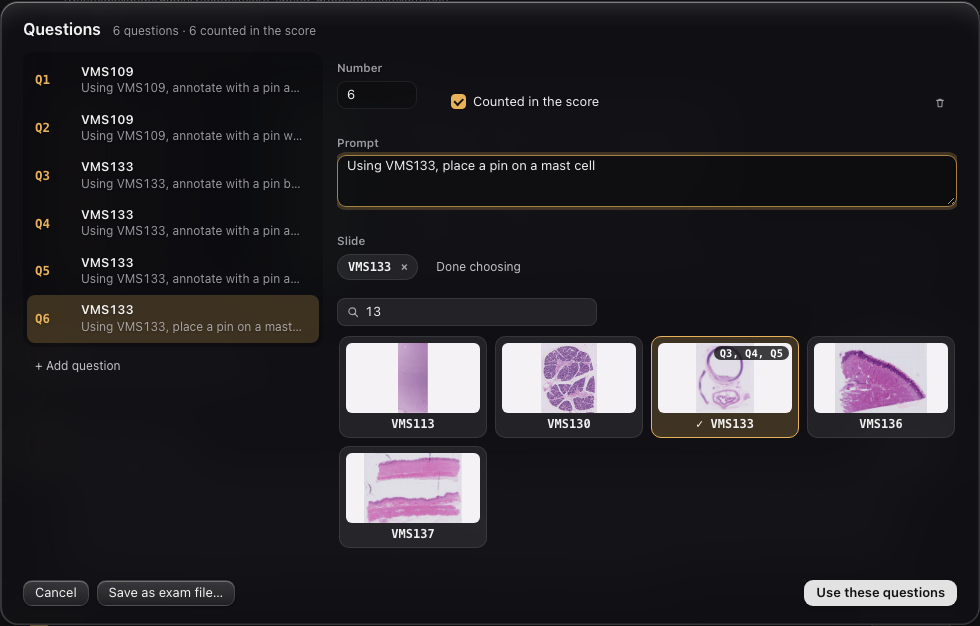
\includegraphics[width=0.7\linewidth, height=4.2cm, keepaspectratio]{img/exam-editor.png}}\par{\scriptsize The question editor}\par}\smallskip
{\small Covers: Before grading starts \textperiodcentered{} Choose slides \textperiodcentered{} Save as an exam file \textperiodcentered{} Inside a session}
\tcblower
\centering\href{https://github.com/agadin/micro-speed-grader/blob/main/docs/help/exam-questions.md}{\qrcode[height=1.75cm, nolink]{https://github.com/agadin/micro-speed-grader/blob/main/docs/help/exam-questions.md}}\\[3pt]\helplink{exam-questions.md}
\end{pagecard}

\begin{pagecard}\phantomsection\addcontentsline{toc}{subsection}{Clusters and navigation}\label{sec:clusters}
{\large\bfseries Clusters and navigation}\par\smallskip
Pins that land near each other are grouped into a \textbf{cluster}. Two settings in the right panel's \textbf{Clusters} section control it:\par

{\small Covers: How clusters work \textperiodcentered{} Moving around \textperiodcentered{} Images \textperiodcentered{} The minimap and scale \textperiodcentered{} Measure distances and areas}
\tcblower
\centering\href{https://github.com/agadin/micro-speed-grader/blob/main/docs/help/clusters.md}{\qrcode[height=1.75cm, nolink]{https://github.com/agadin/micro-speed-grader/blob/main/docs/help/clusters.md}}\\[3pt]\helplink{clusters.md}
\end{pagecard}

\begin{pagecard}\phantomsection\addcontentsline{toc}{subsection}{The ledger and undo}\label{sec:ledger}
{\large\bfseries The ledger and undo}\par\smallskip
The \textbf{Ledger} under the slide lists every grade on this image: one row per group of pins you graded together, with its reason and pin count. Tick \textbf{All images} to see the whole exam.\par
\par\smallskip{\centering\tcbox[enhanced, boxsep=0pt, left=0pt, right=0pt, top=0pt, bottom=0pt, arc=4pt, boxrule=0.5pt, colframe=black, colback=white, clip upper]{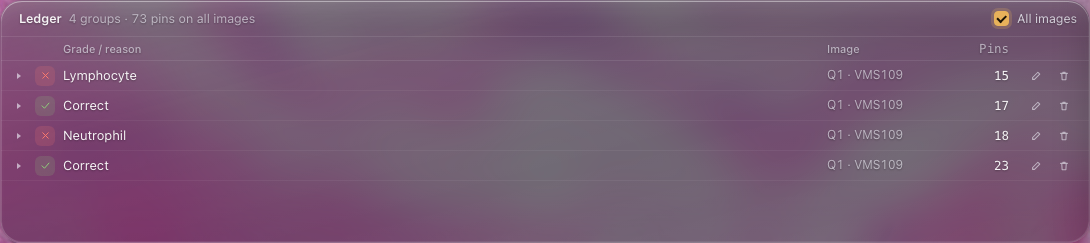
\includegraphics[width=0.7\linewidth, height=4.2cm, keepaspectratio]{img/ledger.png}}\par{\scriptsize The ledger}\par}\smallskip
{\small Covers: What you can do with a row \textperiodcentered{} Search and filter \textperiodcentered{} Undo and redo}
\tcblower
\centering\href{https://github.com/agadin/micro-speed-grader/blob/main/docs/help/ledger.md}{\qrcode[height=1.75cm, nolink]{https://github.com/agadin/micro-speed-grader/blob/main/docs/help/ledger.md}}\\[3pt]\helplink{ledger.md}
\end{pagecard}

\begin{pagecard}\phantomsection\addcontentsline{toc}{subsection}{Look up a student}\label{sec:students}
{\large\bfseries Look up a student}\par\smallskip
When a student asks about their grade, you don't need to hunt image by image. The student panel shows everything about one student: every question, what they answered, who graded it and why, and the feedback they'll get. You can check each pin on the slide and change a grade from there.\par
\par\smallskip{\centering\tcbox[enhanced, boxsep=0pt, left=0pt, right=0pt, top=0pt, bottom=0pt, arc=4pt, boxrule=0.5pt, colframe=black, colback=white, clip upper]{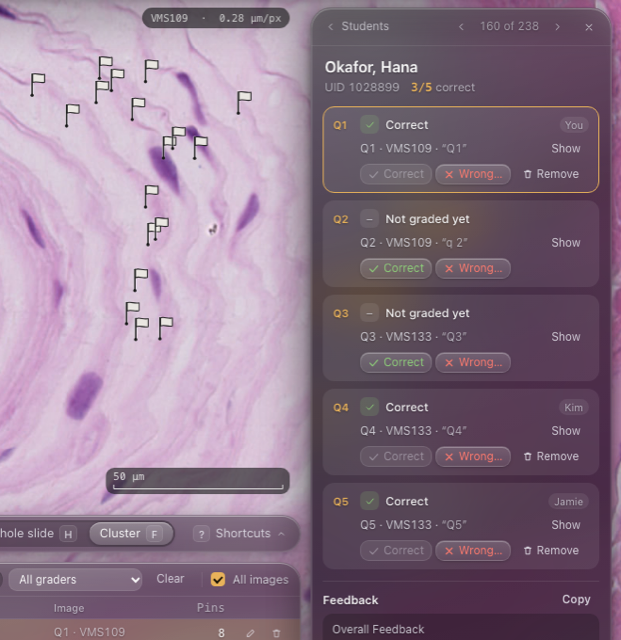
\includegraphics[width=0.7\linewidth, height=4.2cm, keepaspectratio]{img/students.png}}\par{\scriptsize The student panel beside the slide}\par}\smallskip
{\small Covers: Open a student \textperiodcentered{} What it shows \textperiodcentered{} Change a grade}
\tcblower
\centering\href{https://github.com/agadin/micro-speed-grader/blob/main/docs/help/students.md}{\qrcode[height=1.75cm, nolink]{https://github.com/agadin/micro-speed-grader/blob/main/docs/help/students.md}}\\[3pt]\helplink{students.md}
\end{pagecard}

\begin{pagecard}\phantomsection\addcontentsline{toc}{subsection}{What students see}\label{sec:feedback}
{\large\bfseries What students see}\par\smallskip
Every student gets a short feedback note built from your grades. The same text goes into their own \texttt{feedback/\textless{}name\textgreater{}.txt} file and into the \textbf{Comment} column of \texttt{grades.csv}.\par
\par\smallskip{\centering\tcbox[enhanced, boxsep=0pt, left=0pt, right=0pt, top=0pt, bottom=0pt, arc=4pt, boxrule=0.5pt, colframe=black, colback=white, clip upper]{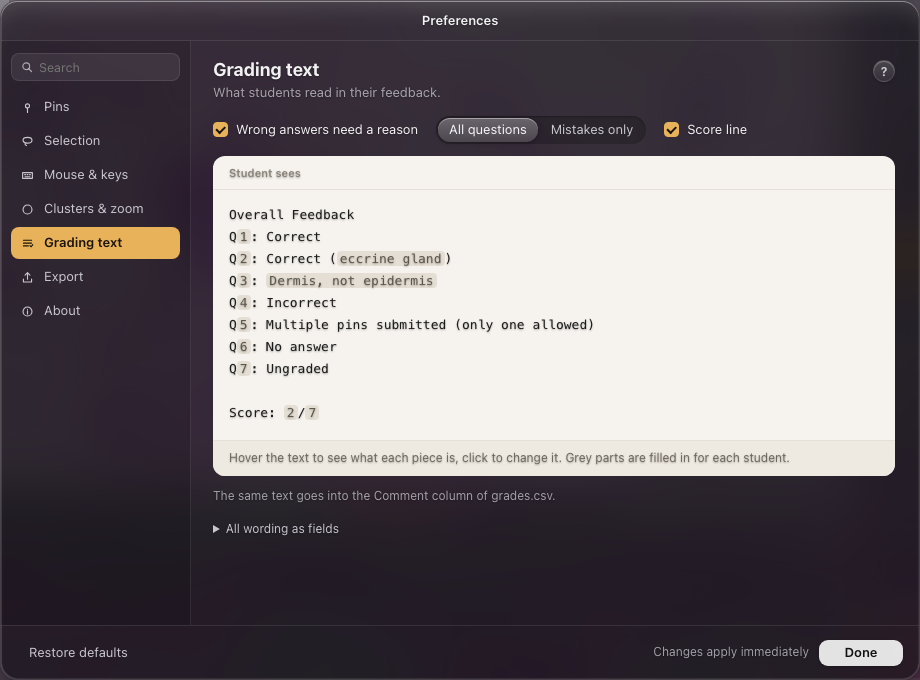
\includegraphics[width=0.7\linewidth, height=4.2cm, keepaspectratio]{img/prefs-text.png}}\par{\scriptsize Editing the feedback wording}\par}\smallskip
{\small Covers: Changing the wording}
\tcblower
\centering\href{https://github.com/agadin/micro-speed-grader/blob/main/docs/help/feedback.md}{\qrcode[height=1.75cm, nolink]{https://github.com/agadin/micro-speed-grader/blob/main/docs/help/feedback.md}}\\[3pt]\helplink{feedback.md}
\end{pagecard}

\begin{pagecard}\phantomsection\addcontentsline{toc}{subsection}{Preferences}\label{sec:preferences}
{\large\bfseries Preferences}\par\smallskip
Open Preferences with \keycap{\cmdsym{}}\keyplus{}\keycap{,} or the gear in the top bar. It opens in its own window; changes apply immediately. Type in the search field at the top of the sidebar to find a setting. \textbf{Restore defaults} resets everything.\par

{\small Covers: Pins \textperiodcentered{} Selection \textperiodcentered{} Mouse \& keys \textperiodcentered{} Clusters \& zoom \textperiodcentered{} Reading submissions \textperiodcentered{} Grading text \textperiodcentered{} Export \textperiodcentered{} About}
\tcblower
\centering\href{https://github.com/agadin/micro-speed-grader/blob/main/docs/help/preferences.md}{\qrcode[height=1.75cm, nolink]{https://github.com/agadin/micro-speed-grader/blob/main/docs/help/preferences.md}}\\[3pt]\helplink{preferences.md}
\end{pagecard}

\begin{pagecard}\phantomsection\addcontentsline{toc}{subsection}{Troubleshooting}\label{sec:troubleshooting}
{\large\bfseries Troubleshooting}\par\smallskip
\textbf{"No questions like ``Q1. Using VMS123, \ldots{}'' were found in that file."} The exam's questions must start like \texttt{Q1. Using VMS109, \ldots{}}. If the PDF is a scan (an image with no text), make a JSON exam file instead:\par

{\small Covers: Setting up a session \textperiodcentered{} While grading \textperiodcentered{} Updates \textperiodcentered{} Still stuck?}
\tcblower
\centering\href{https://github.com/agadin/micro-speed-grader/blob/main/docs/help/troubleshooting.md}{\qrcode[height=1.75cm, nolink]{https://github.com/agadin/micro-speed-grader/blob/main/docs/help/troubleshooting.md}}\\[3pt]\helplink{troubleshooting.md}
\end{pagecard}

\appendix
\section{How pins are matched to questions}\label{app:pins}\label{sec:getting-started:how-student-pins-are-read}

When it reads the submissions folder, the app works out who placed each pin, on which slide, and which question it answers.

\begin{itemize}[topsep=2pt, itemsep=2pt]
\item \textbf{Student.} Each first-level folder in the submissions folder is one student. Its name becomes the student's name, and a number in it becomes their UID.
\item \textbf{Slide.} The slide ID comes from the \texttt{.ndpa} file name (\texttt{VMS109.ndpi.ndpa} is for VMS109).
\item \textbf{Answers.} Pins and shapes (circles, outlines) are answers; a shape counts as a pin at its centre. Rulers, arrows and text notes aren't (see \emph{Count as answers} below).
\item \textbf{Limits.} To stop a damaged file from slowing the app: 2 MB per annotation file, 200 annotations per file and 50 pins per student per slide.
\end{itemize}

\subsection*{Which question a pin answers}

Only the questions that use the pin's slide are considered. The app reads the pin's title (the label the student typed in NDP.view) and tries these rules in order, stopping at the first that gives an answer:

\begin{enumerate}[topsep=2pt, itemsep=2pt]
\item \textbf{The title is just the question}: \emph{Q3}, \emph{q3} or \emph{Q 3}.
\item \textbf{The title names the question} anywhere in it: \emph{Question 3: sweat gland}, \emph{my answer Q3}, \emph{Q\#3}.
\item \textbf{The title has exactly one number that is a question on this slide}: \emph{3}, \emph{\#3}, \emph{pin 3}, \emph{3) sweat gland}. Other numbers are ignored, so \emph{VMS109 \#3} still means Q3 (unless the exam has a question 109 on that slide).
\item \textbf{Nothing in the title decides it.}
\begin{itemize}[topsep=1pt]
\item On a slide that \textbf{only one question uses}, the pin belongs to that question, whatever its title says.
\item On a slide that \textbf{several questions use}, if the student's other pins on that slide already answer all but one of its questions, the pin answers \textbf{the one that's left}. A student who labels one pin \emph{Q3} on a slide used by Q3 and Q13 has their other, unlabelled pin counted as Q13.
\item Otherwise the pin is \emph{unlabelled}: it appears on each question it could answer with a \keycap{?} badge. Grading it under one question assigns it to that question; \textbf{Remove grade} undoes that.
\end{itemize}
\end{enumerate}

A title that names a question the slide isn't for (\emph{Q9} on a slide used only by Q3 and Q13) is listed in \hyperref[sec:getting-started:things-to-check]{Things to check} as \textbf{Pin names a question not on that slide}, and the pin is then placed by rule~4.

\begin{table}[H]\centering
\begin{tabularx}{\linewidth}{@{}l>{\raggedright\arraybackslash}p{0.27\linewidth}Y@{}}
\toprule
\textbf{Pin title} & \textbf{Slide used by Q3 and Q13}\textsuperscript{*} & \textbf{Slide used only by Q5} \\
\midrule
\emph{Q3} & Q3 (rule 1) & Q5 (rule 4); flagged: names Q3 \\
\emph{Question 13 -- duct} & Q13 (rule 2) & Q5 (rule 4); flagged: names Q13 \\
\emph{\#3} or \emph{3} & Q3 (rule 3) & Q5 (rule 4) \\
\emph{3 or 13} & unlabelled \keycap{?} on Q3 and Q13 & Q5 (rule 4) \\
\emph{sweat gland} & unlabelled \keycap{?} on Q3 and Q13 & Q5 (rule 4) \\
\emph{Q9} & unlabelled \keycap{?} on Q3 and Q13; flagged & Q5 (rule 4); flagged \\
\bottomrule
\end{tabularx}
\par\smallskip{\footnotesize\textsuperscript{*}For a student with no other pin on that slide. With the default settings in Preferences \menuarrow{} Reading submissions.}
\caption{Where some pin titles end up}\label{tab:titles}
\end{table}

\subsection*{Changing the rules}

These rules can be changed in \href{https://github.com/agadin/micro-speed-grader/blob/main/docs/help/preferences.md\#reading-submissions}{Preferences \menuarrow{} Reading submissions}\,\onlinemark{}. The defaults are in bold.

\begin{itemize}[topsep=2pt, itemsep=3pt]
\item \textbf{Count as answers}: pins only, \textbf{pins and shapes} (circles and outlines count as a pin at their centre), or every annotation (rulers, arrows and text notes too). With every annotation, a student who measured something in NDP.view has a second ``pin'' for that question.
\item \textbf{Bare numbers} (rule 3): \textbf{on}, or off. Turn it off when titles often contain numbers that aren't question numbers: then only titles that say \emph{Q3} or \emph{question 3} count, and the rest are placed by rule 4.
\item \textbf{Title names another question}: \textbf{use the pin for its slide's question}, or leave the pin out, so the student has no answer for that question unless they have another pin. Either way the pin is listed in Things to check.
\item \textbf{Leftover question} (rule 4): \textbf{on}, or off. Off, a pin is never given to the student's remaining question; it stays unlabelled for you to decide.
\item \textbf{Unlabelled pins} (whatever is still unlabelled after the leftover rule): \textbf{show on each question, with a \keycap{?}}, give them to the lowest-numbered question, or leave them out.
\item \textbf{Several pins for one question}: \textbf{mark them wrong automatically}, or leave them for you to grade. Left for you, the pins keep their \keycap{2} badge but stay ungraded (and count as ungraded in the export) until you grade one of them. Either way, a grade you give one of them is what counts.
\end{itemize}

New sessions use these settings, and each session keeps the ones it was made with, so a later rescan reads it the same way. (Sessions made before version 0.3.8 count every annotation.) Changing a setting while a session is open reads its submissions again with the new rules, after saving a copy of the session next to it. A graded pin that now answers a different question loses its grade for the old one; pins that are left out are set aside with their grades. \textbf{Several pins for one question} applies straight away, without reading anything again. A hand-off pack carries the host's setting, so other graders treat several pins the same way.

\subsection*{More than one pin for a question}

If a student ends up with two or more pins for the same question, by any of the rules above, they're all marked wrong as \emph{Multiple pins submitted (only one allowed)} unless you grade one of them yourself, or set \emph{Several pins for one question} to leave them for you (see \hyperref[sec:grading:double-pins]{Double pins}). An unlabelled \keycap{?} pin doesn't count towards this until it's assigned. Likewise, a student whose only pin for a question is an unlabelled one is shown as ungraded for it (not \emph{No answer}) until you grade that pin.



\end{document}
